\documentclass[12pt,a4paper]{article}
\usepackage[british]{babel}
\usepackage[a4paper,margin=1in]{geometry}
\usepackage[round,authoryear]{natbib}
\usepackage{graphicx,booktabs,multirow,float,caption,subcaption,xcolor,enumitem,tikz,amsmath}
\usetikzlibrary{positioning,arrows.meta,shapes.geometric,calc}
\usepackage{xurl}
\usepackage[hidelinks]{hyperref}
\graphicspath{{../figures/}{../}}
\setlength{\parskip}{4pt}
\setlength{\parindent}{0pt}
\captionsetup{font=small}

\newcommand{\pdash}{-}
\begin{document}

% ------------------------------------------------------------------ title
\begin{titlepage}
\centering
\vspace*{2cm}
{\LARGE\bfseries Analysing the Role of Big Data Analytics for Cyber Threat Detection and Prevention in Banking Organisations of Ireland\par}
\vspace{1.5cm}
{\Large Final Research Project Report\par}
\vspace{1.5cm}
{\large Jayanth Akarapu\par}
\vspace{0.6cm}
Research Practicum, Open Data Practice\par
Supervisor: Dr.\ Prasanth Nayak\par
\vfill
{\large September 2026\par}
\end{titlepage}

% ------------------------------------------------------------------ abstract
\begin{abstract}
Irish banks process a fast-growing volume of digital transactions. Rule-based security controls struggle to keep up with it. This project evaluates how Big Data Analytics can detect and prevent cyber threats and fraud in banking. It compares supervised machine learning models on a public, labelled dataset of bank transactions \citep{kaggle2025dataset}. The dataset has 33{,}611 records, and 42.3\% of them are flagged suspicious.

Following a quantitative experimental design, the study builds one reproducible pipeline. The pipeline covers data cleaning, feature engineering, stratified 80:20 splitting, 5-fold cross-validated hyper-parameter tuning and statistical comparison. It compares the three models in the proposal, Decision Tree, Random Forest and a Support Vector Machine. Logistic Regression, gradient boosting and a transparent two-condition rule serve as baselines.

On the held-out test set, the Decision Tree and the Random Forest perform the same: F1 is 0.996, with a 95\% bootstrap confidence interval of 0.994 to 0.998. Recall is 0.9996 and ROC-AUC is 0.997 to 0.998. Both are significantly better than the SVM (F1 0.989) and Logistic Regression (F1 0.991), with McNemar $p<0.001$. The SVM is also the slowest model, taking about 80 times longer than the Decision Tree to train.

A set of robustness experiments puts these near-perfect scores in context:
\begin{itemize}[nosep]
\item A two-condition rule learnt from the training data reaches F1 0.995: \emph{merchant has a suspicious history} and \emph{amount $>$ 197{,}827}. The labels therefore follow a nearly deterministic pattern.
\item Removing merchant information lowers F1 to 0.80.
\item For merchants that the model never saw in training, F1 falls to 0.86 to 0.88.
\end{itemize}

Big Data Analytics works best in this setting as a way to find and then operationalise simple, auditable risk patterns. Black-box accuracy on its own adds little here. The report ends with recommendations for Irish banks that link these findings to GDPR, DORA and the EU AI Act.

\medskip
\textbf{Keywords:} Big Data Analytics, cybersecurity, banking, fraud detection, machine learning, explainability, Ireland
\end{abstract}

\newpage
\tableofcontents
\newpage

% ================================================================== 1
\section{Introduction}

\subsection{Research background}
Online, mobile and instant payments have changed Irish retail banking. Faster and more convenient services have also widened the attack surface. Phishing, account takeover, malware, data breaches and authorised-push-payment fraud are now everyday risks for banks and their customers.

Cybercrime was projected to cost the world economy about \$10.5 trillion a year by 2025 \citep{cybersecurityventures2020}. In Ireland, almost 90\% of companies reported disruption or financial loss from cyberattacks in 2025 \citep{irishtimes2025}. Banks hold large amounts of money and sensitive personal data, so they are frequent targets. When they are breached, they suffer financial loss and regulatory sanctions. They also lose customer trust.

Big Data Analytics (BDA) means collecting, storing and analysing large, fast-moving and varied data. It has become a core defensive capability. Platforms such as Hadoop and Spark \citep{zaharia2016spark}, used together with machine learning (ML) libraries in Python \citep{pedregosa2011scikit, niazi2024bigdata}, let banks score every transaction. These tools can find anomalous behaviour and adapt to new attack patterns faster than static rule sets \citep{buczak2016survey, ofoegbu2024realtime}.

\subsection{Problem statement}
Traditional signature-based and rule-based controls are good at catching known, simple attacks. They struggle with the volume of modern transaction streams and with sophisticated or evolving fraud. The literature shows that ML-based detection works well on generic cybersecurity benchmarks \citep{ahmad2021network, hozouri2025comprehensive}. There is much less evidence on the following two points:
\begin{enumerate}[label=(\roman*)]
\item how established, interpretable ML models compare on \emph{banking transaction} data;
\item what that means for banks that operate under Irish and EU regulation.
\end{enumerate}

\subsection{Aim, objectives and research questions}
\textbf{Aim.} To analyse the role of Big Data Analytics in detecting and preventing cyber threats in banking organisations in Ireland.

\textbf{Objectives.}
\begin{enumerate}[nosep]
\item Identify how BDA is used to detect current cyber threats faced by banking organisations.
\item Evaluate the effectiveness of BDA techniques, namely machine learning and predictive analytics, for identifying and mitigating cyber threats.
\item Identify the challenges of implementing BDA in banking institutions.
\item Recommend strategies for successful implementation of BDA in Irish banks.
\end{enumerate}

\textbf{Research questions.}
\begin{description}[nosep,leftmargin=1.2cm,labelwidth=1cm]
\item[RQ1] How is Big Data Analytics used to detect and prevent cyber threats in banking organisations in Ireland?
\item[RQ2] How effective are BDA-based techniques, such as machine learning and predictive analytics, at identifying and mitigating cyber threats?
\item[RQ3] What challenges do banking institutions face when implementing BDA?
\item[RQ4] Which strategies can banking institutions adopt to implement BDA successfully?
\end{description}

\subsection{Contributions}
\begin{enumerate}[nosep]
\item A fully reproducible, open-source pipeline covering EDA, feature engineering, tuning, evaluation and explainability. It compares Decision Tree, Random Forest and SVM against three reference models on a public banking dataset.
\item A statistically grounded comparison: 5-fold cross-validation, bootstrap confidence intervals and McNemar tests.
\item A robustness analysis that the proposal did not plan: rule baseline, feature ablation, re-balancing, temporal split and unseen-merchant generalisation. It shows \emph{why} the models score so highly and where they would fail.
\item Practical, regulation-aware recommendations for Irish banks.
\end{enumerate}

\subsection{Structure of the report}
\begin{itemize}[nosep]
\item Section~\ref{sec:lit} reviews related work.
\item Section~\ref{sec:method} describes the methodology.
\item Section~\ref{sec:design} presents the design and Section~\ref{sec:impl} the implementation.
\item Section~\ref{sec:eval} reports the results.
\item Section~\ref{sec:disc} discusses them against the research questions.
\item Section~\ref{sec:concl} concludes.
\end{itemize}

% ================================================================== 2
\section{Related Work}\label{sec:lit}

\subsection{Big Data Analytics in cybersecurity}
\citet{buczak2016survey} surveyed data-mining and ML methods for intrusion detection. They showed that hidden patterns in large security datasets support better detection than hand-written signatures. \citet{martinez2019machine} argued that ML reduces reliance on rule-based approaches by automating threat detection. They also warned that results depend on good data and features.

\citet{ofoegbu2024realtime} described how streaming BDA platforms combined with ML enable real-time threat detection in high-volume environments. \citet{zaharia2016spark} set out the distributed-computing engine that makes such workloads practical. \citet{kumar2025bigdata} tested ML models on 500{,}000 security incidents and reported 96.8\% accuracy for deep learning, 94.1\% for Random Forest and 92.3\% for SVM, with 35\% fewer false positives when big data analytics was combined with blockchain. \citet{kokogho2025fintech} reviewed how predictive modelling and behaviour analytics support cyber risk management in fintech.

Banking brings its own constraints: strict latency limits, heavy regulation, and a high cost for false alarms. \citet{sathupadi2025banknet} addressed these directly with BankNet, which combines Apache Spark and Kafka with a BiLSTM model to score internet banking transactions in real time. It reached 98.5\% fraud detection accuracy at up to 1000 Mbps. It is the closest example of a big data architecture built for banking, and it guides the design side of this project.

\subsection{Machine learning for cyber threat detection}
Early deep-learning IDS work \citep{javaid2016deep, vinayakumar2019deep} and hybrid CNN-LSTM designs \citep{khan2019scalable} showed accuracy gains over classical IDS. The systematic study by \citet{ahmad2021network} found that ML and deep learning beat conventional security strategies consistently. It also listed recurring problems: class imbalance, computational cost and model maintenance.

\citet{hozouri2025comprehensive} reviewed a large body of IDS research, covering signature-, anomaly- and hybrid-based detection. They named adversarial robustness, real-time latency, scalability, explainability (SHAP, LIME) and imbalanced data as open challenges.

\citet{zhang2025intelligent} built an ensemble of deep networks on the BoT-IoT dataset. The ensemble reached 99.985\% accuracy and 99.54\% F1. These results are impressive, but they come from network-traffic benchmarks, not financial transactions.

\subsection{Intrusion detection systems and datasets}
\citet{ring2019survey} and \citet{ferrag2020deep} showed that published detection performance depends heavily on the dataset. Many benchmark datasets are dated, synthetic or unrepresentative, and models tuned on them may not transfer to real deployments. This point is central to the present study. Section~\ref{sec:eval} tests directly how far performance on a public transaction dataset reflects a learnable, general signal rather than dataset artefacts.

Privacy is another IDS concern. \citet{laddi2025federated} proposed a federated-learning IDS in which organisations train collaboratively without pooling raw data. It reached 94.16\% accuracy and 93.82\% F1. This design is attractive under GDPR \citep{gdpr2016}.

\citet{pospichal2026rf} show how a Random Forest IDS should be evaluated carefully. On UNSW-NB15 they combined mutual-information feature selection, randomised hyper-parameter search and SMOTE, and reported F1 between 0.93 and 0.98 across five attack types. Their protocol of tuning on training data only and reporting per-class F1 is followed in this study.

\subsection{Cyber threat intelligence and predictive analytics}
\citet{montasari2020application} argued that AI and ML turn large volumes of security telemetry into actionable cyber threat intelligence. This supports proactive rather than reactive defence.

\citet{padmanaban2026actp} proposed a banking-specific framework, the Automated Cyber Threat Detection and Prevention (ACTP) tool. It combines reinforcement learning, ethical-hacking simulation and adversarial training. The tool reported 88.2\% accuracy and a 5.1\% false-positive rate. This highlights that attackers adapt, and that robustness matters as much as accuracy on a static test set. \citet{kovacevic2025ai} make the same point conceptually, describing data poisoning and evasion attacks against banking AI and the dual use of AI by attackers.

\citet{eshra2025threat} studied threat intelligence in financial institutions and reported that more mature threat intelligence was associated with 33.7\% lower breach likelihood and 28\% faster incident response. \citet{ullah2026risk} proposed a risk assessment framework for US banks with a hybrid XGBoost and LSTM model (96.4\% accuracy, ROC-AUC 0.982), although on simulated data.

\subsection{Big Data Analytics in banking security and fraud detection}
\citet{hasan2023bigdata} reviewed Big Data in banking operations. They found clear benefits for fraud monitoring and risk management, along with persistent concerns about privacy, regulation and governance. The systematic review of ML-based financial fraud detection by \citet{ali2022financial} covered 93 articles and found that credit card fraud is the most studied fraud type and that SVM and artificial neural networks are the most popular algorithms.

Recent banking studies point to tree ensembles. \citet{sanda2026banking} compared Logistic Regression, Random Forest, SVM, gradient boosting and a neural network on a Kaggle banking fraud dataset with SMOTE and a 70:15:15 split; Random Forest was best with 97.2\% accuracy and 98.4\% AUC. \citet{dhammayogi2026early} compared Random Forest, XGBoost and SVM under extreme imbalance and found ROC-AUC of 0.992, 0.995 and 0.935 respectively, with SHAP showing transaction frequency and amount spikes as the key features. \citet{baisholan2025fraudx} combined Random Forest and XGBoost with threshold tuning and SHAP on credit card data, reaching 95\% recall and 97\% AUC-PR.

\citet{naeem2026mlfraud} compared rule-based, ML and AI-driven fraud detection in digital banking. In their simulated set-ups, gradient boosting (XGBoost) scored best, ahead of Random Forest, SVM and Logistic Regression. They stressed explainability for regulators. Their results are based on a \emph{theoretical simulation} rather than real transactions, which reinforces the need for empirical comparisons on actual transaction data.

\subsection{Research gap}
Table~\ref{tab:lit} summarises the most relevant studies. Three gaps motivate this project:
\begin{enumerate}[nosep]
\item few studies compare interpretable classical models (DT, RF, SVM) on \emph{banking transaction} data using rigorous statistical tests;
\item almost none check whether very high reported scores survive tests aimed at dataset artefacts, such as ablation, temporal splits or unseen merchants;
\item Irish or EU banking regulation is rarely linked to the technical results.
\end{enumerate}

\begin{table}[H]
\centering\small
\caption{Summary of key related work.}\label{tab:lit}
\resizebox{\linewidth}{!}{\begin{tabular}{p{3.2cm}p{3.3cm}p{3.6cm}p{4.2cm}}
\toprule
Study & Domain / data & Method & Key limitation for this project \\
\midrule
\citet{buczak2016survey} & Generic IDS & Survey of data mining / ML & Not banking-specific \\
\citet{ahmad2021network} & Network IDS & ML vs DL systematic study & Imbalance, maintenance cost \\
\citet{hozouri2025comprehensive} & IDS benchmarks & Survey (ML, DL, XAI) & No banking focus \\
\citet{zhang2025intelligent} & BoT-IoT & DL ensemble + SMOTE & Network traffic, not transactions \\
\citet{laddi2025federated} & Network IDS & Federated ML & No banking data \\
\citet{sathupadi2025banknet} & Internet banking & BiLSTM with Spark and Kafka & Deep model, hard to audit \\
\citet{pospichal2026rf} & UNSW-NB15 & RF, feature selection, SMOTE & Network traffic, not transactions \\
\citet{sanda2026banking} & Banking fraud & LR, RF, SVM, GB, NN & Accuracy-led reporting \\
\citet{dhammayogi2026early} & Digital banking & RF, XGBoost, SVM, SHAP & No rule baseline \\
\citet{padmanaban2026actp} & Banking attacks & Adversarial ML and RL & Lower accuracy (88.2\%) \\
\citet{ali2022financial} & Financial fraud & Systematic review & No new experiments \\
\citet{naeem2026mlfraud} & Digital banking & RF, XGB, SVM, LR & Simulated results only \\
\bottomrule
\end{tabular}}
\end{table}

% ================================================================== 3
\section{Research Methodology}\label{sec:method}

\subsection{Research design}
The study uses a \emph{quantitative experimental} design on secondary data. The unit of analysis is a single bank transaction and the outcome is the binary label \texttt{isSuspicious}. Models are the experimental treatments. Performance metrics on unseen data are the dependent variables. All randomness is controlled by a fixed seed (42), so every result can be regenerated exactly.

\subsection{Dataset}
The \emph{Bank Transaction Records along Suspicious Flags} dataset \citep{kaggle2025dataset} was downloaded with the Kaggle API. It contains 33{,}611 transactions dated 16~December~2022 to 12~January~2025. There are six raw fields:
\begin{itemize}[nosep]
\item \texttt{date};
\item \texttt{description}, a narrative such as \texttt{NETTXN:AMAZON} or \texttt{CRYPTOEXCHANGEBINANCE};
\item \texttt{debit}, \texttt{credit} and \texttt{balance};
\item the label \texttt{isSuspicious}.
\end{itemize}

There are no missing values and no duplicate rows. The 43 distinct descriptions fall into 10 transaction channels. 14{,}203 transactions (42.3\%) are suspicious, so the classes are only mildly imbalanced (Figure~\ref{fig:eda}a).

The dataset is public, anonymised and synthetic in style: account numbers are clearly placeholders. It contains no data about real individuals.

\subsection{Pre-processing and feature engineering}
Table~\ref{tab:features} lists the engineered features. Numeric features are standardised and categorical features are one-hot encoded. Both steps run inside a scikit-learn \texttt{Pipeline}, so all transformations are fitted on the training folds only. This prevents information leaking from the test data.

\begin{table}[H]
\centering\small
\caption{Engineered features.}\label{tab:features}
\begin{tabular}{p{4.2cm}p{10cm}}
\toprule
Feature(s) & Definition / rationale \\
\midrule
\texttt{amount}, \texttt{log\_amount} & $\text{debit}+\text{credit}$ and its $\log(1+x)$; transaction size is a classic fraud signal. \\
\texttt{is\_debit} & Direction of money flow. \\
\texttt{balance}, \texttt{log\_balance} & Account balance after the transaction (signed log). \\
\texttt{amount\_to\_balance}, \texttt{negative\_balance} & Size relative to the account and overdraft indicator. \\
\texttt{year}, \texttt{month}, \texttt{day}, \texttt{dayofweek}, \texttt{is\_weekend} & Calendar context. \\
\texttt{channel} & Prefix of the description (e.g.\ NETTXN, PCA, IMPS, CRYPTOEXCHANGE). \\
\texttt{description} & Full merchant / narrative (43 levels). \\
\bottomrule
\end{tabular}
\end{table}

\subsection{Models}
Three models come from the proposal:
\begin{itemize}[nosep]
\item \textbf{Decision Tree} (CART) \citep{breiman1984classification}: interpretable if-then rules.
\item \textbf{Random Forest} \citep{breiman2001random}: a bagged ensemble of 300 trees.
\item \textbf{Support Vector Machine} with an RBF kernel \citep{cortes1995support}.
\end{itemize}

Three reference models put these results in context:
\begin{itemize}[nosep]
\item \textbf{Logistic Regression}, a linear baseline;
\item \textbf{Histogram Gradient Boosting} \citep{friedman2001greedy}, a state-of-the-art tabular learner;
\item a \textbf{Rule baseline}, which flags a transaction when both hold: its description has any suspicious history in the training data, and its amount exceeds a threshold chosen to maximise training F1.
\end{itemize}
The rule baseline mimics a traditional, analyst-written control. It shows how much the ML models add beyond it.

Class imbalance is handled with \texttt{class\_weight="balanced"}. Section~\ref{sec:imb} compares this with SMOTE \citep{chawla2002smote} and with no re-balancing.

\subsection{Evaluation protocol}
\begin{enumerate}[nosep]
\item \textbf{Hold-out split.} Stratified 80:20 split: 26{,}888 training and 6{,}723 test transactions.
\item \textbf{Tuning.} Grid search with 5-fold stratified CV on the training set, optimising F1. The grids are:
\begin{itemize}[nosep]
\item Decision Tree: depth $\{5,10,20,\infty\}$ and minimum leaf size $\{1,5,20\}$;
\item Random Forest: depth $\{10,20,\infty\}$ and minimum leaf size $\{1,5\}$;
\item SVM: $C\in\{0.1,1,10\}$ and $\gamma\in\{\text{scale},0.01\}$.
\end{itemize}
\item \textbf{Metrics.} Accuracy, precision, recall, F1, ROC-AUC, PR-AUC \citep{saito2015precision} and the confusion matrix. A 1{,}000-sample bootstrap gives the 95\% CI for test F1.
\item \textbf{Significance.} Exact McNemar tests between the best model and every other model \citep{dietterich1998approximate}.
\item \textbf{Robustness.}
\begin{itemize}[nosep]
\item feature-group ablation;
\item re-balancing strategies;
\item a \emph{temporal} split: train before 17~March~2024, test on or after that date;
\item \emph{unseen-merchant} generalisation: 5-fold \texttt{GroupKFold} over descriptions, without the description feature.
\end{itemize}
\item \textbf{Explainability and operations.}
\begin{itemize}[nosep]
\item Random Forest impurity importance and SHAP values \citep{lundberg2017unified};
\item decision-threshold trade-off;
\item training time as data size grows, and scoring latency per transaction.
\end{itemize}
\end{enumerate}

\subsection{Ethical considerations}
The research uses only public, anonymised, secondary data, so no human participants were involved and no informed consent was needed. The data is used only for academic purposes, and no attempt is made to identify people or organisations.

Model bias and fairness were considered. The label is only mildly imbalanced, and re-balancing is tested explicitly. The limitations of synthetic data for real-world claims are stated openly in Section~\ref{sec:limits}. Any production use would require a Data Protection Impact Assessment under GDPR Article~35 \citep{gdpr2016}. It would also require governance of high-risk AI under the EU AI Act \citep{euaiact2024}.

% ================================================================== 4
\section{Design Specification}\label{sec:design}
Figure~\ref{fig:arch} shows the analytics architecture. The experimental core (solid boxes) is implemented in this project. The dashed boxes show how the same trained pipeline would sit inside a bank's big-data stack:
\begin{itemize}[nosep]
\item transactions stream in through Kafka or Spark;
\item each one is scored in real time by the serialised model;
\item alerts go to the fraud or SOC team;
\item analyst feedback is fed back as new labels.
\end{itemize}

\begin{figure}[H]
\centering
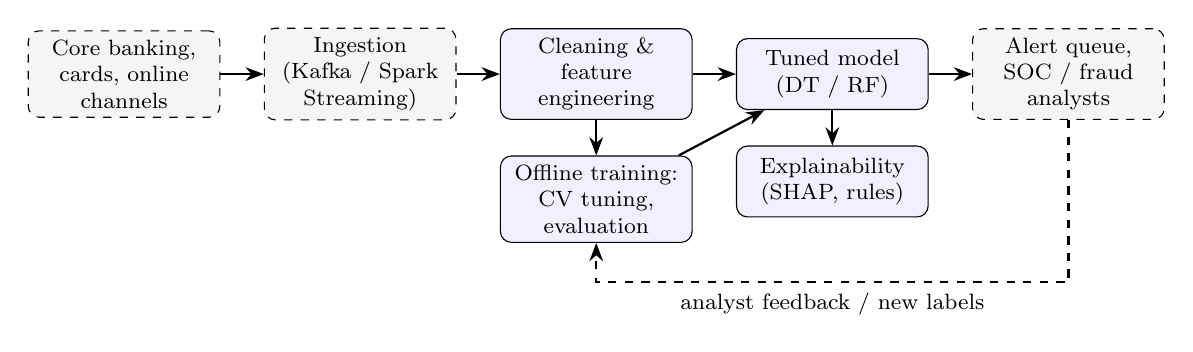
\begin{tikzpicture}[node distance=0.45cm and 0.55cm, font=\footnotesize,
  box/.style={draw, rounded corners, fill=blue!6, minimum height=0.9cm, align=center, text width=2.2cm},
  ext/.style={box, dashed, fill=gray!8},
  arr/.style={-{Stealth}, thick}]
\node[ext] (src) {Core banking,\\ cards, online\\ channels};
\node[ext, right=of src] (ing) {Ingestion\\ (Kafka / Spark\\ Streaming)};
\node[box, right=of ing] (prep) {Cleaning \&\\ feature\\ engineering};
\node[box, right=of prep] (model) {Tuned model\\ (DT / RF)};
\node[ext, right=of model] (alert) {Alert queue,\\ SOC / fraud\\ analysts};
\node[box, below=of prep] (train) {Offline training:\\ CV tuning,\\ evaluation};
\node[box, below=of model] (xai) {Explainability\\ (SHAP, rules)};
\draw[arr] (src) -- (ing); \draw[arr] (ing) -- (prep); \draw[arr] (prep) -- (model); \draw[arr] (model) -- (alert);
\draw[arr] (prep) -- (train); \draw[arr] (train) -- (model); \draw[arr] (model) -- (xai);
\draw[arr, dashed] (alert.south) |- node[pos=.75, below]{analyst feedback / new labels} ($(train.south)+(0,-0.5)$) -- (train.south);
\end{tikzpicture}
\caption{Proposed Big Data Analytics architecture. Solid boxes are implemented; dashed boxes show deployment context.}\label{fig:arch}
\end{figure}

% ================================================================== 5
\section{Implementation}\label{sec:impl}
The work was implemented in Python~3 with pandas, NumPy, scikit-learn~1.5 \citep{pedregosa2011scikit}, imbalanced-learn, statsmodels, SHAP, Matplotlib and Seaborn. The project repository is organised as follows:
\begin{itemize}[nosep]
\item \texttt{src/pipeline.py}: the complete, single-command experiment (EDA $\rightarrow$ tuning $\rightarrow$ evaluation $\rightarrow$ robustness $\rightarrow$ figures). It takes about four minutes on a 15-core laptop.
\item \texttt{notebooks/analysis.ipynb}: an executed Jupyter notebook that reruns the pipeline and shows every table and figure.
\item \texttt{results/}: machine-readable outputs (CSV/JSON) for every table in this report.
\item \texttt{figures/}: all figures.
\end{itemize}

Every pre-processing step sits inside the model pipeline, which prevents leakage from the test data. Grid search, cross-validation and Random Forest training run in parallel on all CPU cores (\texttt{n\_jobs=-1}). This is the single-node equivalent of the data-parallel execution that Spark provides on a cluster.

% ================================================================== 6
\section{Evaluation}\label{sec:eval}

\subsection{Exploratory data analysis}
Figure~\ref{fig:eda} summarises the data. Suspicious activity is concentrated in a few channels:
\begin{itemize}[nosep]
\item crypto-exchange purchases: 71.8\% suspicious;
\item online (NETTXN) payments such as travel booking and e-commerce: 61.4\%;
\item card (PCA) purchases at online retailers.
\end{itemize}
ATM withdrawals, cash deposits, EMI repayments, IMPS transfers, refunds and salary credits are never flagged. Within the risky channels, suspicious transactions are much larger: every transaction below roughly 200{,}000 currency units is normal. The suspicious share also varies over time. It peaks in 2023 at 50.2\%, against 19.5\% in 2024.

\begin{figure}[H]
\centering
\begin{subfigure}{0.32\textwidth}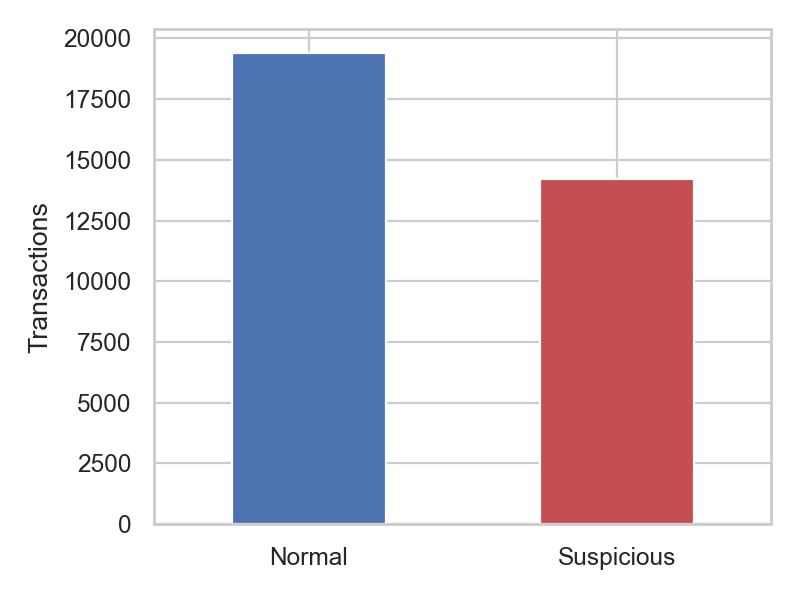
\includegraphics[width=\linewidth]{class_balance}\caption{Class balance}\end{subfigure}
\begin{subfigure}{0.66\textwidth}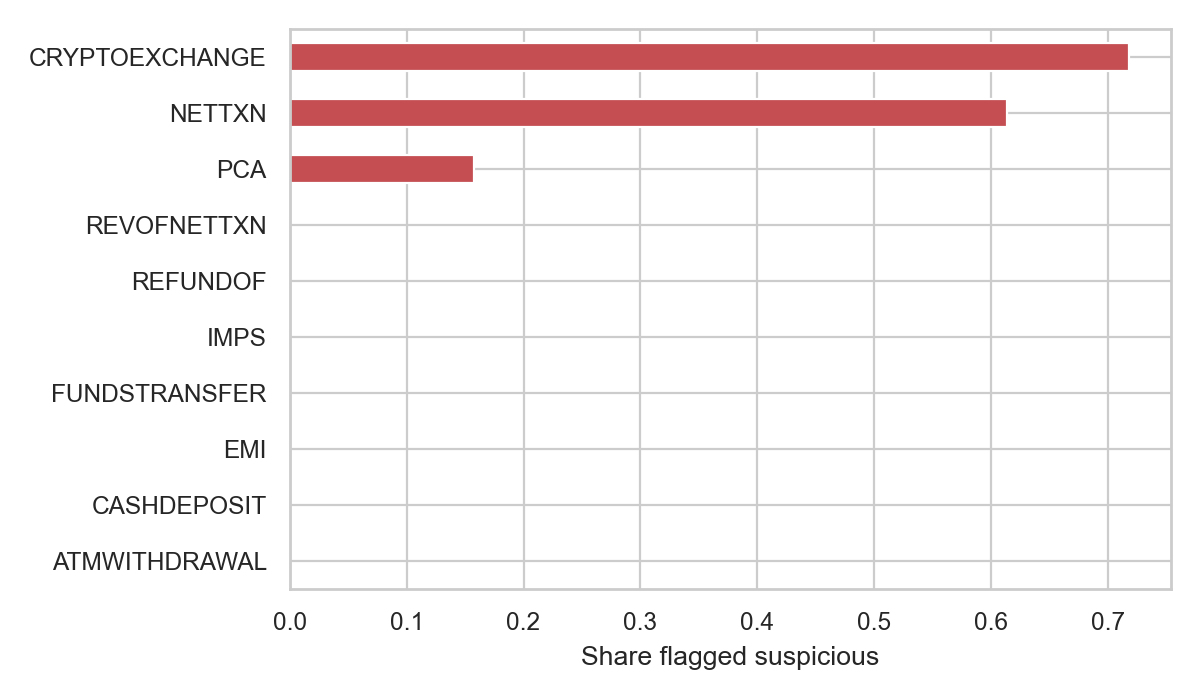
\includegraphics[width=\linewidth]{suspicious_rate_by_channel}\caption{Suspicious share by channel}\end{subfigure}\\[4pt]
\begin{subfigure}{0.48\textwidth}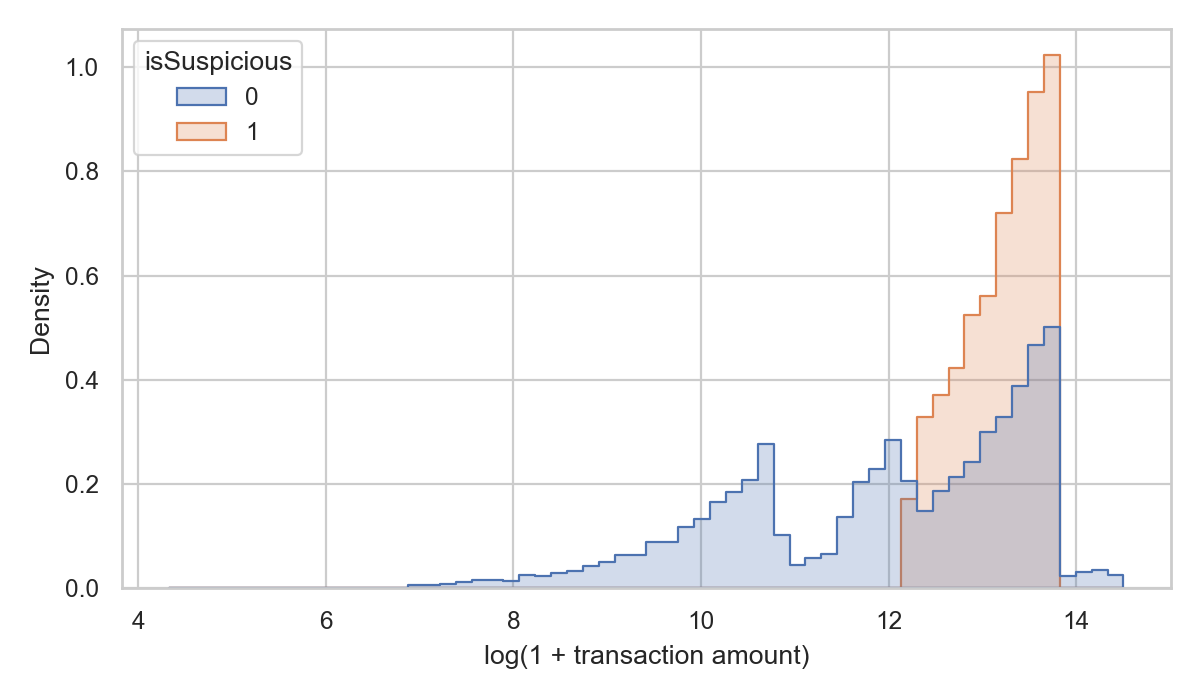
\includegraphics[width=\linewidth]{amount_distribution}\caption{Amount distribution by class}\end{subfigure}
\begin{subfigure}{0.50\textwidth}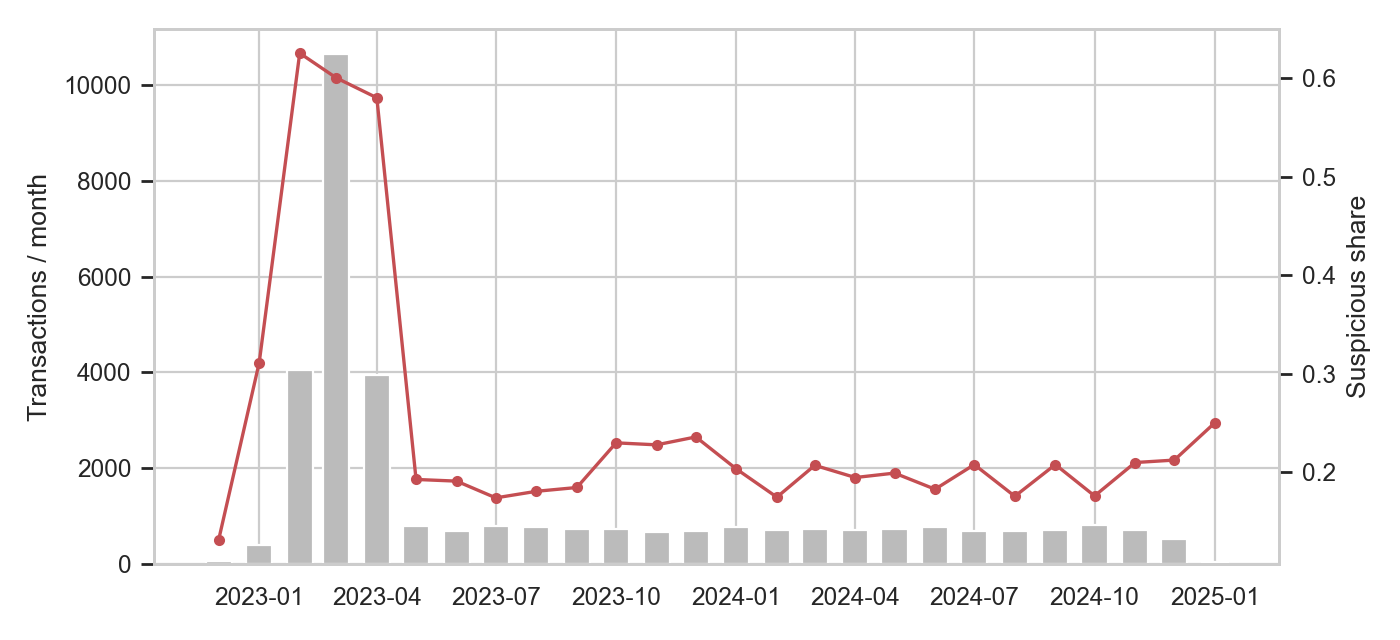
\includegraphics[width=\linewidth]{monthly_trend}\caption{Monthly volume and suspicious share}\end{subfigure}
\caption{Exploratory analysis of the 33{,}611 transactions.}\label{fig:eda}
\end{figure}

\subsection{Model comparison}
Table~\ref{tab:tuning} shows the selected hyper-parameters. Table~\ref{tab:test} and Figure~\ref{fig:comp} report performance on the held-out test set.

\begin{table}[H]
\centering\small
\caption{Selected hyper-parameters (5-fold CV, F1).}\label{tab:tuning}
\begin{tabular}{lll}
\toprule
Model & Best parameters & CV F1 \\
\midrule
Decision Tree & max\_depth = 10, min\_samples\_leaf = 5 & 0.9963 \\
Random Forest & max\_depth = 20, min\_samples\_leaf = 1 & 0.9963 \\
SVM (RBF) & $C = 10$, $\gamma$ = scale & 0.9874 \\
\bottomrule
\end{tabular}
\end{table}

\begin{table}[H]
\centering\small
\caption{Test-set performance ($n=6{,}723$; 2{,}841 suspicious). Latency is per transaction, measured for batch scoring. Rule-baseline AUCs are computed from hard labels.}\label{tab:test}
\resizebox{\linewidth}{!}{\begin{tabular}{lcccccccc}
\toprule
Model & Acc. & Prec. & Rec. & F1 [95\% CI] & ROC-AUC & PR-AUC & FP & FN \\
\midrule
Decision Tree & \textbf{0.9966} & \textbf{0.9923} & 0.9996 & \textbf{0.9960} [0.994, 0.998] & 0.9976 & 0.9938 & 22 & 1 \\
Random Forest & \textbf{0.9966} & \textbf{0.9923} & 0.9996 & \textbf{0.9960} [0.994, 0.998] & 0.9971 & 0.9938 & 22 & 1 \\
Gradient Boosting & 0.9964 & 0.9916 & \textbf{1.0000} & 0.9958 [0.994, 0.997] & \textbf{0.9987} & \textbf{0.9977} & 24 & 0 \\
Rule baseline & 0.9958 & 0.9902 & \textbf{1.0000} & 0.9951 [0.993, 0.997] & 0.9964 & 0.9902 & 28 & 0 \\
Logistic Regression & 0.9924 & 0.9830 & 0.9993 & 0.9911 [0.989, 0.994] & 0.9965 & 0.9913 & 49 & 2 \\
SVM (RBF) & 0.9909 & 0.9857 & 0.9930 & 0.9893 [0.987, 0.992] & 0.9965 & 0.9911 & 41 & 20 \\
\bottomrule
\end{tabular}}
\end{table}

\begin{figure}[H]
\centering
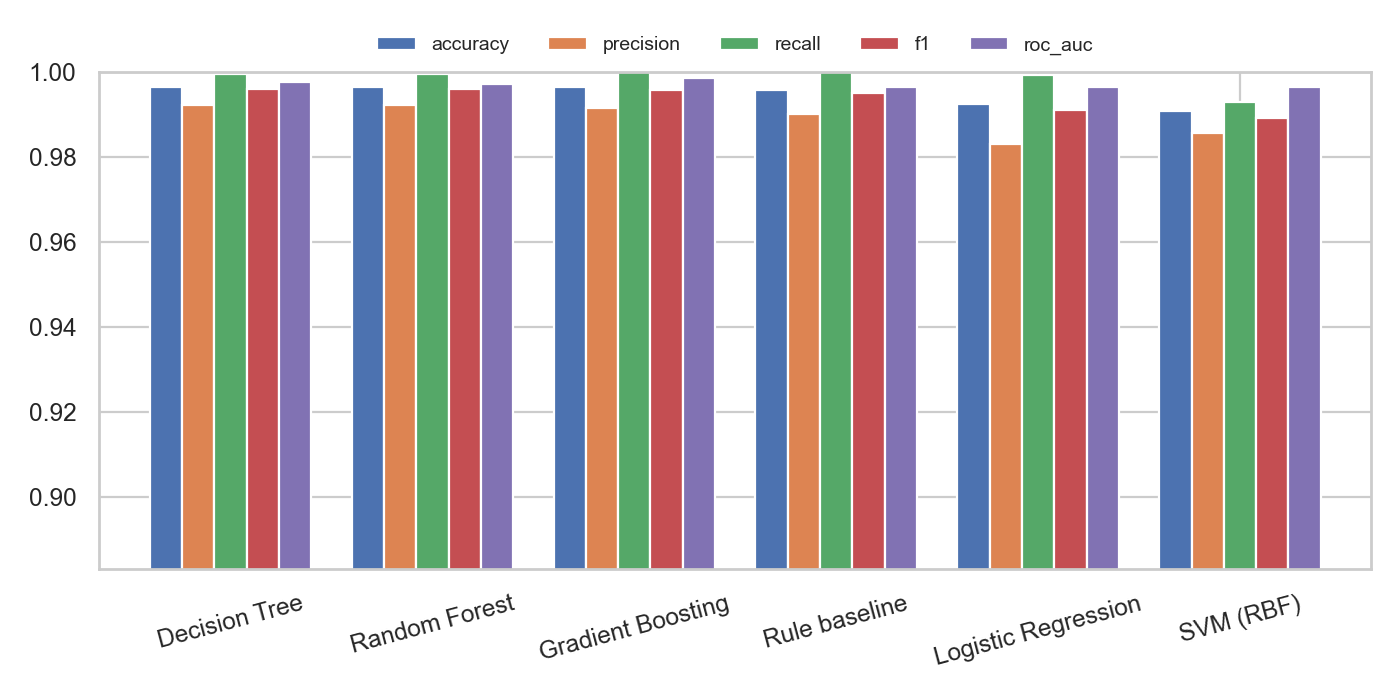
\includegraphics[width=0.85\linewidth]{model_comparison}
\caption{Test-set metrics by model (note the truncated y-axis).}\label{fig:comp}
\end{figure}

All models are highly accurate. The two tree-based models from the proposal make exactly the same predictions on the test set: 22 false alarms and a single missed suspicious transaction out of 2{,}841. Gradient boosting misses none but raises two extra false alarms, and it has the best ranking quality (ROC-AUC 0.9987). The SVM is clearly the weakest of the proposal's models. It misses 20 suspicious transactions, twenty times as many as the tree models.

Figure~\ref{fig:roc} shows the ROC and precision-recall curves, and Figure~\ref{fig:cm} the confusion matrices.

\begin{figure}[H]
\centering
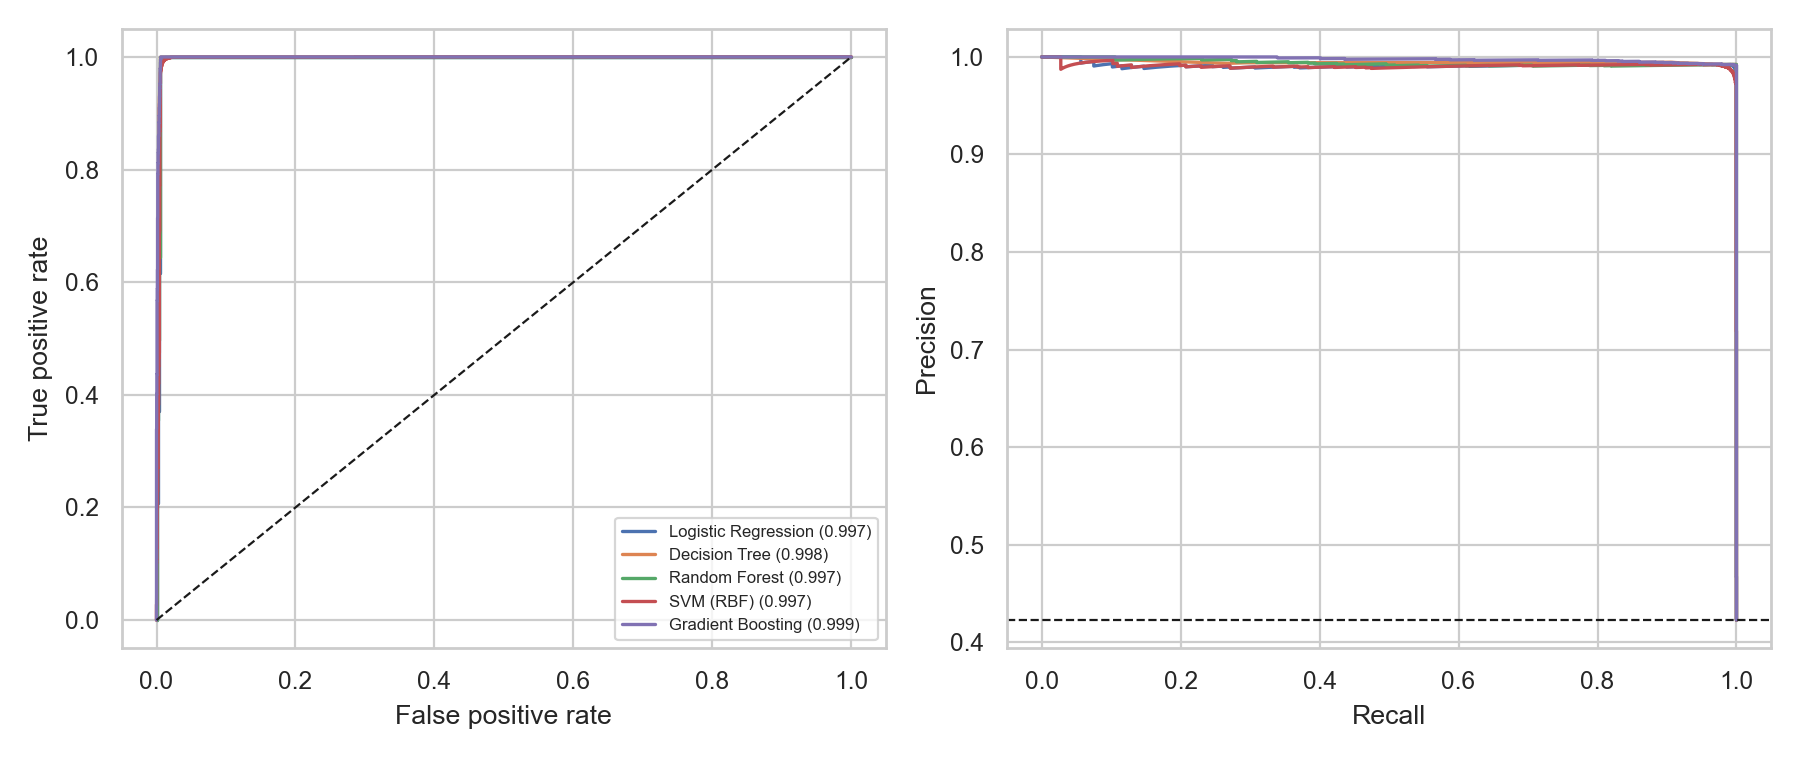
\includegraphics[width=0.95\linewidth]{roc_pr_curves}
\caption{ROC (left) and precision-recall (right) curves on the test set. The dashed line on the right is the prevalence baseline.}\label{fig:roc}
\end{figure}

\begin{figure}[H]
\centering
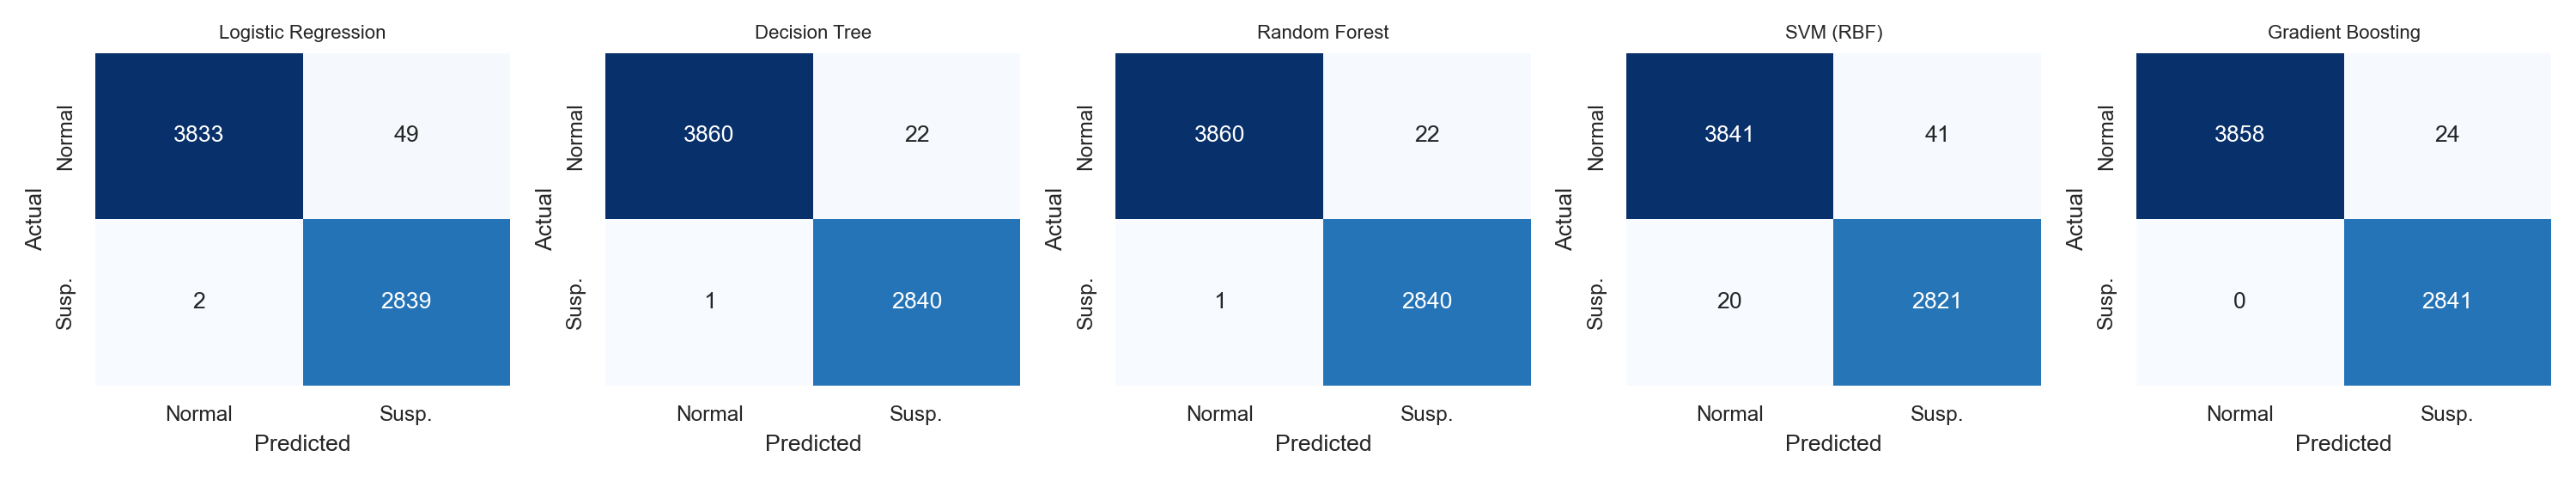
\includegraphics[width=\linewidth]{confusion_matrices}
\caption{Confusion matrices (rows: actual; columns: predicted).}\label{fig:cm}
\end{figure}

\subsection{Cross-validation and statistical significance}
Table~\ref{tab:cv} confirms that the hold-out ranking is stable across folds. The standard deviations are at most 0.0014 F1.

Exact McNemar tests (Table~\ref{tab:mcnemar}) show that the Decision Tree is significantly better than the SVM and Logistic Regression ($p<0.001$). Where the Decision Tree and the SVM disagree, the tree is right 39 times and the SVM once. The Decision Tree is \emph{not} distinguishable from Random Forest, whose predictions are identical, or from Gradient Boosting ($p=1.0$).

\begin{table}[H]
\centering\small
\begin{minipage}{0.54\textwidth}\centering
\caption{5-fold CV on the training set (mean $\pm$ sd).}\label{tab:cv}
\resizebox{\linewidth}{!}{\begin{tabular}{lcc}
\toprule
Model & F1 & ROC-AUC \\
\midrule
Decision Tree & 0.9963 $\pm$ 0.0012 & 0.9980 $\pm$ 0.0007 \\
Random Forest & 0.9963 $\pm$ 0.0012 & 0.9972 $\pm$ 0.0009 \\
Gradient Boosting & 0.9952 $\pm$ 0.0010 & 0.9983 $\pm$ 0.0005 \\
Logistic Reg. & 0.9900 $\pm$ 0.0014 & 0.9971 $\pm$ 0.0009 \\
SVM (RBF) & 0.9874 $\pm$ 0.0006 & 0.9971 $\pm$ 0.0009 \\
\bottomrule
\end{tabular}}
\end{minipage}\hfill
\begin{minipage}{0.43\textwidth}\centering
\caption{McNemar tests vs Decision Tree.}\label{tab:mcnemar}
\resizebox{\linewidth}{!}{\begin{tabular}{lccc}
\toprule
Other & DT only & Other only & $p$ \\
\midrule
Log.\ Reg. & 29 & 1 & $<$0.001 \\
Random Forest & 0 & 0 & 1.00 \\
SVM (RBF) & 39 & 1 & $<$0.001 \\
Grad.\ Boost. & 2 & 1 & 1.00 \\
\bottomrule
\end{tabular}}
\end{minipage}
\end{table}

\subsection{What drives the performance? Rule baseline and ablation}\label{sec:ablation}
Scores near 99.6\% F1 call for scrutiny. A two-condition rule, learnt from the training data, reaches F1 0.9951 on the test set, only 0.0009 below the best model:
\begin{center}
\emph{flag if the description has any suspicious history \textbf{and} amount $>$ 197{,}827}
\end{center}
It never misses a suspicious transaction and raises only 28 false alarms. The labels in this dataset therefore follow a nearly deterministic pattern: \emph{large transactions in risk-prone merchant categories}. The ML models learn that pattern with slightly fewer false positives.

The feature-group ablation with Random Forest (Table~\ref{tab:ablation}) confirms this. Merchant/channel information and amount are both necessary, and neither is sufficient on its own:
\begin{itemize}[nosep]
\item Removing description/channel drops F1 from 0.996 to 0.800.
\item Amount and balance alone reach only 0.745.
\item Description/channel alone reaches 0.839. Recall is perfect, but precision is poor.
\item Calendar features add nothing (F1 unchanged at 0.996), despite the visible drift in the suspicious rate over time.
\end{itemize}

\begin{table}[H]
\centering\small
\caption{Feature-group ablation (Random Forest, same split).}\label{tab:ablation}
\begin{tabular}{lcccc}
\toprule
Feature set & Precision & Recall & F1 & ROC-AUC \\
\midrule
All features & 0.9923 & 0.9996 & 0.9960 & 0.9971 \\
Without date features & 0.9923 & 0.9996 & 0.9960 & 0.9976 \\
Description / channel only & 0.7223 & 1.0000 & 0.8388 & 0.8615 \\
Without description / channel & 0.8160 & 0.7849 & 0.8001 & 0.8904 \\
Amount \& balance only & 0.6020 & 0.9761 & 0.7447 & 0.7718 \\
\bottomrule
\end{tabular}
\end{table}

\subsection{Class-imbalance handling}\label{sec:imb}
Random Forest gives the same F1 of 0.9960 with no re-balancing, with balanced class weights and with SMOTE. PR-AUC ranges only from 0.9923 to 0.9939. At a 42:58 class ratio, re-balancing is not needed. This contrasts with real card-fraud data, where fraud is often well below 1\% of transactions and re-balancing matters a lot \citep{zhang2025intelligent, ali2022financial}.

\subsection{Temporal robustness}
In production, a model is trained on the past and used on the future. The models were therefore retrained on transactions before 17~March~2024 and tested on all later ones. The later period has a much lower suspicious rate, 19.6\%.

The tree models and gradient boosting hold up fully: F1 is 0.999 to 1.000. The SVM with calendar features degrades sharply: F1 falls to 0.855 and recall to 0.750. Once calendar features are removed, its F1 recovers to 0.994.

\emph{Calendar features are a liability for drift-sensitive models.} Year and month encode the historic base rate, and that rate changes over time. For deployment, they should be left out or monitored.

\subsection{Generalisation to unseen merchants}
The hardest test holds out whole merchant descriptions, using 5-fold \texttt{GroupKFold}. The model must then judge transactions at merchants it has never seen, using only channel, amount, balance and date. Table~\ref{tab:group} shows that F1 falls to 0.86 to 0.88 and varies more across folds (sd $\approx$ 0.05). The ranking quality stays good, with ROC-AUC 0.95 to 0.97.

Gradient boosting and Random Forest generalise best. This is the most realistic estimate of how the models would handle a new e-commerce or crypto platform, and it shows why continuous retraining matters.

\begin{table}[H]
\centering\small
\caption{Unseen-merchant generalisation (GroupKFold over 43 descriptions, 5 folds, mean).}\label{tab:group}
\begin{tabular}{lcccc}
\toprule
Model & Precision & Recall & F1 ($\pm$ sd) & ROC-AUC \\
\midrule
Gradient Boosting & 0.9018 & 0.8618 & \textbf{0.8776} $\pm$ 0.053 & \textbf{0.9741} \\
Random Forest & 0.8778 & 0.8677 & 0.8694 $\pm$ 0.050 & 0.9735 \\
Decision Tree & 0.8436 & 0.8787 & 0.8584 $\pm$ 0.046 & 0.9629 \\
SVM (RBF) & 0.8416 & 0.8800 & 0.8573 $\pm$ 0.040 & 0.9528 \\
\bottomrule
\end{tabular}
\end{table}

\subsection{Explainability}
Figure~\ref{fig:xai} shows the global explanation of the Random Forest. Transaction amount (raw and log-scaled) is the most important feature, followed by the NETTXN and CRYPTOEXCHANGE channel indicators. SHAP values show the direction of each effect:
\begin{itemize}[nosep]
\item high amounts and crypto or online-payment channels push towards \emph{suspicious};
\item IMPS transfers, salary credits and local-shop card payments push towards \emph{normal}.
\end{itemize}
These explanations match the rule baseline. A compliance officer could check them easily, which is what regulators expect \citep{euaiact2024}.

\begin{figure}[H]
\centering
\begin{subfigure}{0.46\textwidth}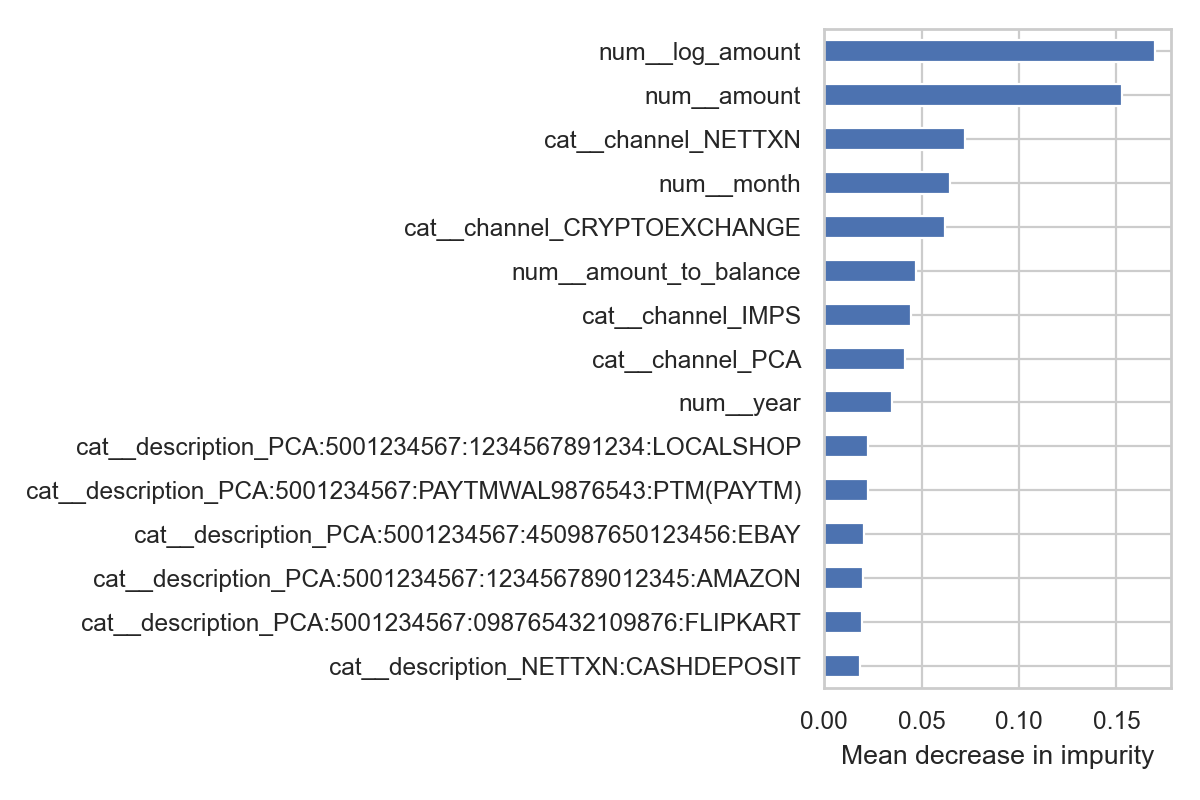
\includegraphics[width=\linewidth]{rf_feature_importance}\caption{Impurity-based importance}\end{subfigure}
\begin{subfigure}{0.52\textwidth}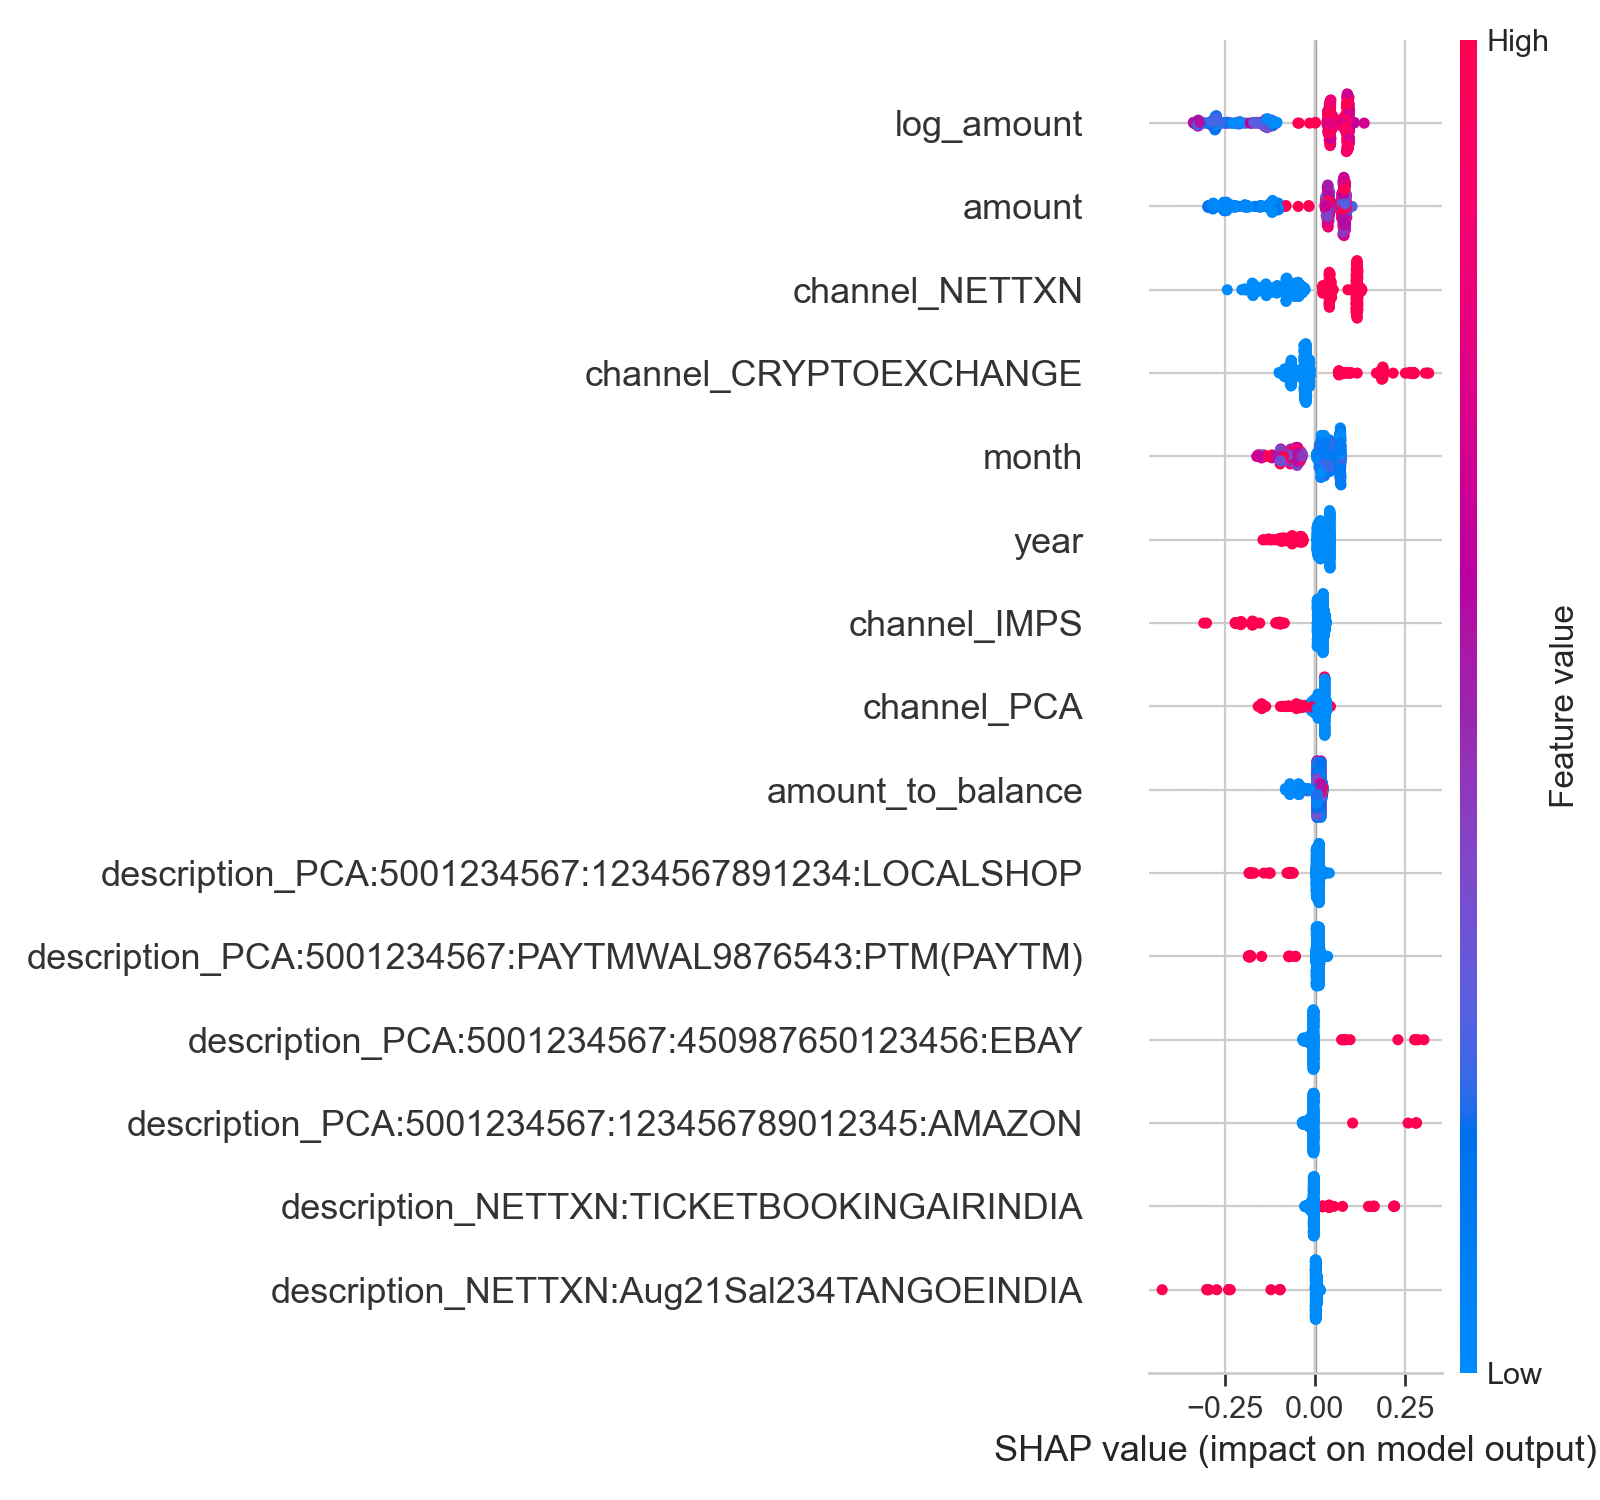
\includegraphics[width=\linewidth]{shap_summary}\caption{SHAP summary (500 test transactions)}\end{subfigure}
\caption{Global explanations of the Random Forest.}\label{fig:xai}
\end{figure}

\subsection{Operational trade-offs: threshold, latency and scalability}
For the Decision Tree, precision and recall stay flat across decision thresholds from 0.10 to 0.65 (Figure~\ref{fig:ops}a). The model is very confident, so the alert volume, about 426 per 1{,}000 transactions in this dataset, is set by the data rather than by the threshold.

Training time (Figure~\ref{fig:ops}b) grows roughly linearly for the tree models: 0.09\,s for the Decision Tree and 0.42\,s for the Random Forest on 26{,}888 rows. For the SVM it grows super-linearly: 0.2\,s at 10\% of the data, but 7.4\,s at 100\%, a 35-fold increase for 10 times the data. Scoring latency is below 0.01\,ms per transaction for the tree models and about 0.07\,ms for the SVM.

At bank scale, with millions of transactions a day, these costs favour tree ensembles. Kernel SVMs would need approximation or distributed training.

\begin{figure}[H]
\centering
\begin{subfigure}{0.49\textwidth}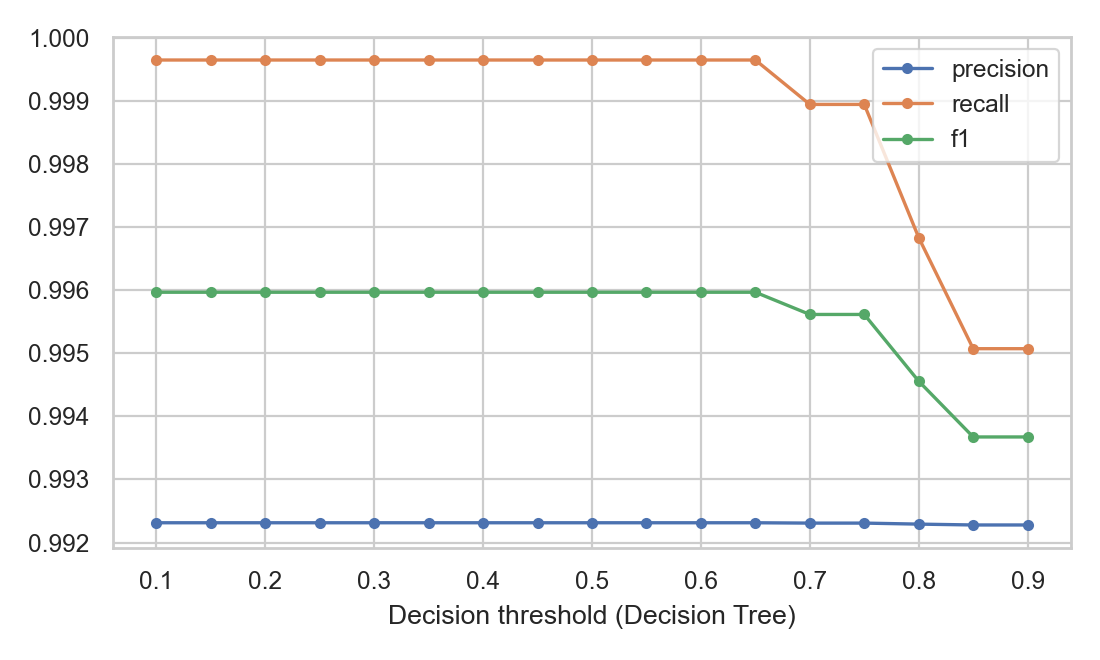
\includegraphics[width=\linewidth]{threshold_tradeoff}\caption{Threshold trade-off (Decision Tree)}\end{subfigure}
\begin{subfigure}{0.46\textwidth}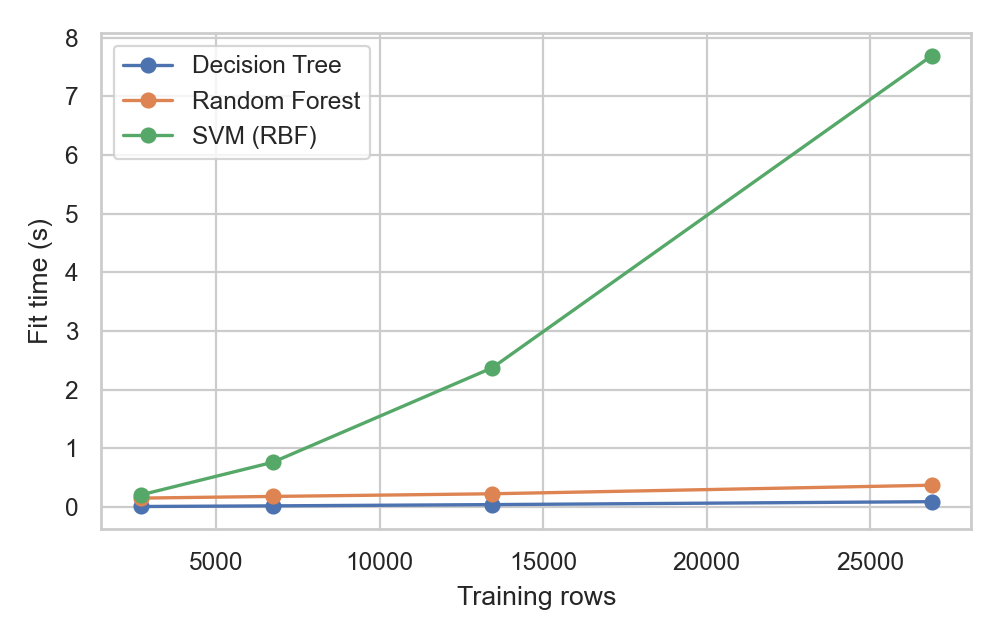
\includegraphics[width=\linewidth]{scalability}\caption{Training time vs data size}\end{subfigure}
\caption{Operational characteristics.}\label{fig:ops}
\end{figure}

% ================================================================== 7
\section{Discussion}\label{sec:disc}

\subsection{RQ1: How is BDA used to detect and prevent cyber threats in banking?}
The literature and the experiments point to three complementary uses:
\begin{enumerate}[label=(\alph*)]
\item \emph{Pattern discovery.} Analysing all transactions, rather than samples, revealed that risk is concentrated in specific channels (crypto and online payments) and at high amounts (Figure~\ref{fig:eda}).
\item \emph{Automated scoring.} Supervised models score each transaction in microseconds and flag it for review. Prevention comes from holding or stepping up authentication on a transaction before it settles.
\item \emph{Intelligence and feedback.} Analyst decisions become new labels, closing the loop described by \citet{montasari2020application} and shown in Figure~\ref{fig:arch}.
\end{enumerate}
Irish banks already run such capabilities in their fraud and SOC functions. This study provides a transparent, reproducible template for them.

\subsection{RQ2: How effective are ML and predictive analytics?}
On this dataset they are very effective:
\begin{itemize}[nosep]
\item Decision Tree and Random Forest reach F1 0.996 and recall 0.9996, significantly better than the SVM and Logistic Regression;
\item gradient boosting reaches the best ROC-AUC;
\item the tree models are also the fastest.
\end{itemize}
This agrees with the reviews that favour tree-based models for tabular fraud data \citep{ali2022financial, naeem2026mlfraud}.

The robustness analysis also shows the limits. A simple rule comes within 0.001 F1 of the best model, and performance drops to about 0.87 F1 on unseen merchants. Headline accuracies above 99\%, common in the literature, should therefore be read as properties of the dataset as much as of the algorithm \citep{ring2019survey}. The real value of ML here lies in three things:
\begin{itemize}[nosep]
\item slightly fewer false alarms than the rule (22 against 28);
\item smoother generalisation to new merchants than a lookup rule, which by construction cannot flag an unseen merchant at all;
\item automatic re-learning as patterns change.
\end{itemize}

\subsection{RQ3: What are the implementation challenges?}
The experiments and the literature point to the following challenges:
\begin{itemize}[nosep]
\item \textbf{Data quality and representativeness.} Public data is synthetic and simplified. Real data is siloed and subject to GDPR \citep{hasan2023bigdata, gdpr2016}.
\item \textbf{Concept drift.} The suspicious rate moved from 50\% in 2023 to 20\% in 2024. Drift-sensitive models (the SVM with calendar features) lost 14 F1 points.
\item \textbf{Generalisation to new attack surfaces.} Unseen merchants reduced F1 by about 13 points.
\item \textbf{Explainability and accountability.} Regulators and customers need reasons for blocked payments, and the EU AI Act \citep{euaiact2024} adds transparency obligations.
\item \textbf{Scalability.} Kernel methods scale poorly. Big-data platforms such as Spark \citep{zaharia2016spark} and skills to run them are needed.
\item \textbf{Adversaries adapt.} Attackers adapt to detectors \citep{padmanaban2026actp}, and static test sets do not show this.
\item \textbf{Class imbalance in real fraud.} Real fraud is far rarer than in this dataset \citep{zhang2025intelligent}.
\end{itemize}

\subsection{RQ4: Recommended strategies for Irish banks}
\begin{enumerate}[nosep]
\item \textbf{Start interpretable, then ensemble.} Deploy tree-based models, whose explanations regulators can audit (SHAP and extracted rules). Keep the analyst rule as a benchmark and a fallback control.
\item \textbf{Evaluate as you deploy.} Report temporal and unseen-segment performance, not just random-split accuracy. Monitor drift, retrain on a schedule, and avoid features that only encode historic base rates.
\item \textbf{Build a governed data platform.} Use streaming ingestion with feature stores on Spark or Kafka, and role-based access. Run a Data Protection Impact Assessment under GDPR Art.~35. Align ICT-risk testing and incident reporting with DORA \citep{dora2022}.
\item \textbf{Collaborate without sharing raw data.} Federated learning \citep{laddi2025federated} lets Irish banks pool fraud intelligence while keeping data local.
\item \textbf{Close the loop.} Feed analyst outcomes back as labels, and red-team the models with adversarial scenarios \citep{padmanaban2026actp}.
\item \textbf{Invest in skills.} Build data-engineering, ML-ops and model-risk-management capacity. Hasan et al.\ identify gaps in these areas as a key barrier \citep{hasan2023bigdata}.
\end{enumerate}

\subsection{Limitations}\label{sec:limits}
\begin{itemize}[nosep]
\item \textbf{The dataset is synthetic in style and not Irish.} Merchant names and channels (e.g.\ IMPS) suggest an Indian retail-banking template. The findings therefore say how BDA \emph{would} work for an Irish bank; they are not a measurement of Irish banks' actual performance.
\item \textbf{The labels are almost deterministic.} Absolute scores overstate real-world performance, as shown in Section~\ref{sec:ablation}.
\item \textbf{No cluster deployment was run.} A Java runtime for Spark was not available in the project environment. Scalability was therefore assessed on a single node with multi-core parallelism.
\item \textbf{No adversarial evaluation or customer-level features.} Features such as velocity and device fingerprinting were not possible with six raw fields.
\end{itemize}

% ================================================================== 8
\section{Conclusion and Future Work}\label{sec:concl}
This project analysed the role of Big Data Analytics in detecting and preventing cyber threats in banking. It built a reproducible experimental pipeline on 33{,}611 labelled bank transactions.

Decision Tree and Random Forest were the most effective and efficient of the proposed models (F1 0.996, recall 0.9996). They were significantly better than the SVM, which was also the least scalable. Gradient boosting matched them and gave the best ranking quality.

The robustness experiments are the main academic contribution. They show that the near-perfect scores come from a simple, explainable pattern: large transactions in crypto and online-payment channels. They also show that performance is much lower for unseen merchants, and that calendar features create drift risk.

For Irish banks, BDA delivers most when it is used to \emph{discover}, \emph{explain} and \emph{operationalise} risk patterns under strong governance, rather than as a black-box accuracy engine.

\textbf{Future work} should:
\begin{enumerate}[label=(\roman*),nosep]
\item validate the pipeline on real, highly imbalanced Irish or EU transaction data under a data-sharing agreement;
\item deploy it on Spark Structured Streaming and measure end-to-end latency;
\item add customer-level behavioural features and graph features linking accounts;
\item evaluate adversarial robustness and federated training across institutions.
\end{enumerate}

\newpage
\bibliographystyle{plainnat}
\bibliography{refs}

\newpage
\appendix
\section{Reproducibility Guide}
\begin{enumerate}[nosep]
\item Install Python 3.10+ and the required packages:\\ {\footnotesize\texttt{pip install pandas numpy scikit-learn imbalanced-learn}\\\texttt{statsmodels shap matplotlib seaborn kaggle}}.
\item Put a Kaggle API token in \texttt{\textasciitilde/.kaggle/} (never commit it). Then run:\\ {\footnotesize\texttt{kaggle datasets download -d}\\\texttt{charanmaik/bank-transaction-records-along-suspicious-flags --unzip -p data}}.
\item Run \texttt{python src/pipeline.py}, which takes about four minutes. All tables are written to \texttt{results/} and all figures to \texttt{figures/}.
\item Optionally, open \texttt{notebooks/analysis.ipynb} to view the results interactively.
\item Build this report with \texttt{cd report \&\& latexmk -pdf thesis.tex}.
\end{enumerate}

\section{Project Plan}
Figure~\ref{fig:gantt} shows the original project schedule. All phases (literature review, data collection, pre-processing, model development, evaluation, analysis and report writing) have been completed.

\begin{figure}[H]
\centering
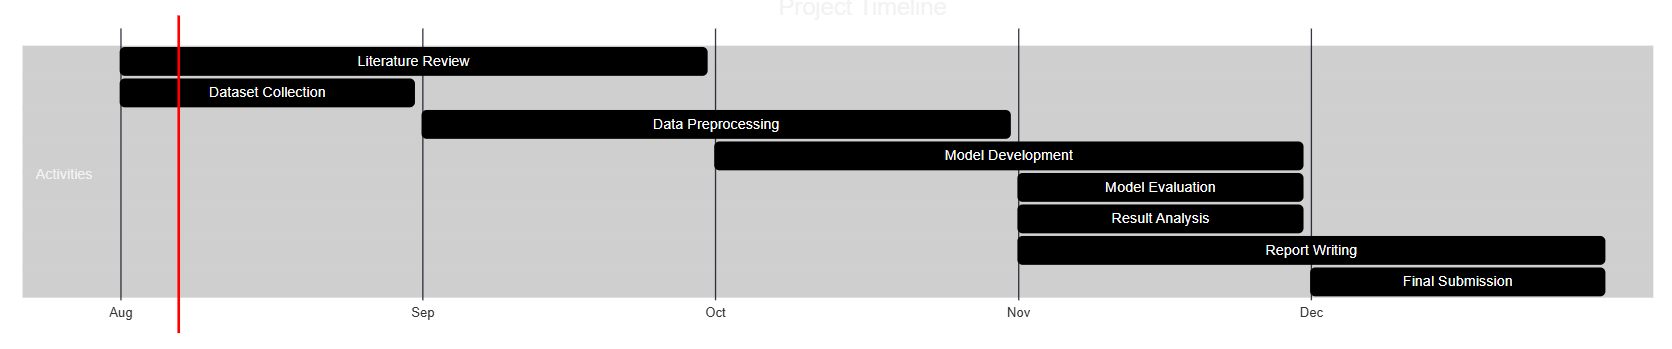
\includegraphics[width=\linewidth]{gantt_chart}
\caption{Project Gantt chart.}\label{fig:gantt}
\end{figure}

\end{document}
